\subsection{变量含误差的回归}\label{sec:12.2}\index{SI0407@变量含误差的回归}
变量含误差的回归（EIV），又称测量误差模型（measurement error model），与\autoref{sec:11.3}的简单线性回归有根本差异，最好把它看成完全不同的主题. 这里将其作为通常回归模型的推广，主要出于传统原因. 然而，这一模型引出的问题很不相同.

本节模型在以下意义上推广简单线性回归：仍处理形如
\begin{equation}\label{eq:12.2.1}Y_i=\alpha+\beta x_i+\varepsilon_i,\end{equation}
的模型，但不再假定$x$已知. 相反，可以测量一个均值为$x_i$的随机变量. （为符合既定符号约定，将把所测随机变量记为$X_i$，其均值记为$\xi_i$，而非$x_i$.）

\sourcepageanchor{499}
这里旨在展示处理EIV模型的不同方法，给出一些标准解法及其有时令人意外的困难. 更全面的介绍可参阅\hyperref[bib:source147]{Gleser（1991）}的综述、\hyperref[bib:source130]{Fuller（1987）}及\hyperref[bib:source62]{Carroll、Ruppert和Stefanski（1995）}的专著，以及\hyperref[bib:source55]{Brown和Fuller（1991）}主编的文集. \hyperref[bib:source189]{Kendall和Stuart（1979}，第29章）也较详细地讨论了这个主题.

一般EIV模型假设观测到成对数据$(x_i,y_i)$，它们来自随机变量$(X_i,Y_i)$，其均值满足线性关系
\begin{equation}\label{eq:12.2.2}EY_i=\alpha+\beta(EX_i).\end{equation}
若定义
$$EY_i=\eta_i\quad\text{和}\quad EX_i=\xi_i,$$
则\eqref{eq:12.2.2}成为
\begin{equation}\label{eq:12.2.3}\eta_i=\alpha+\beta\xi_i,\end{equation}
即随机变量均值之间的线性关系.

变量$\xi_i,\eta_i$有时称为潜变量（latent variables），指不能直接测量的量.\index{SI0602@潜在变量}\semanticindexanchor{602:499} 潜变量不仅可能无法直接测量，甚至可能根本无法测量. 例如，人的智商IQ无法测量. 我们可以测量智商测试的分数，但永远无法测量IQ这个变量. 然而，人们常常假定IQ与其他变量存在关系.

\eqref{eq:12.2.2}所规定的模型实际上没有区分$X$与$Y$. 但若关心回归，就应有理由选择$Y$为响应、$X$为预测变量. 牢记这一关于$Y$对$X$回归的规定，把变量含误差模型或测量误差模型定义如下：按照
\begin{equation}\label{eq:12.2.4}
\begin{aligned}Y_i&=\alpha+\beta\xi_i+\varepsilon_i,&\varepsilon_i&\sim\mathrm n(0,\sigma_\varepsilon^2),\\
X_i&=\xi_i+\delta_i,&\delta_i&\sim\mathrm n(0,\sigma_\delta^2)
\end{aligned}
\end{equation}
观测$(X_i,Y_i)$，$i=1,\ldots,n$.

注意，正态性假设虽然常见，却并非必要. 也可采用其他分布. 实际上，这一模型遇到的一些问题正由正态性假设造成. （例如见\hyperref[bib:source295]{Solari，1969}.）

\begin{example}[估计大气压]\label{ex:12.2.1}
当$x$变量与$y$变量一起被观测，而不是受控制时，EIV回归模型会很自然地出现. 例如，19世纪苏格兰物理学家J. D. Forbes试图用水的沸点测量值估计海拔. 为此，他同时测量沸点和大气压，后者可用于得到海拔. 由于19世纪的气压计十分易损，若能从温度估计气压，更确切地说，估计$\log(\text{气压})$，就会很有用. 在九个地点观测的数据如下，对这种情形采用EIV模型是合理的.
\begin{center}\begin{tabular}{rr}\toprule
沸点（$^\circ\mathrm F$）&$\log(\text{气压})$（$\log(\mathrm{Hg})$）\\\midrule
194.5&1.3179\\197.9&1.3502\\199.4&1.3646\\200.9&1.3782\\201.4&1.3806\\203.6&1.4004\\209.5&1.4547\\210.7&1.4630\\212.2&1.4780\\\bottomrule
\end{tabular}\end{center}
\end{example}

\sourcepageanchor{500}
已经见过模型\eqref{eq:12.2.4}的若干特殊情形. 若$\delta_i=0$，模型就成为简单线性回归，因为此时没有测量误差，可以直接观测$\xi_i$. 若$\alpha=0$，则有
$$\begin{aligned}Y_i&\sim\mathrm n(\eta_i,\sigma_\varepsilon^2),&i&=1,\ldots,n,\\
X_i&\sim\mathrm n(\xi_i,\sigma_\delta^2),&i&=1,\ldots,n,
\end{aligned}$$
其中可能$\sigma_\delta^2\ne\sigma_\varepsilon^2$，这是Behrens--Fisher问题的一个版本.\index{SI0087@Behrens–Fisher问题}\semanticindexanchor{87:500}

\subsubsection{函数关系与结构关系}\label{sec:12.2.1}
EIV模型可规定两类不同的关系：函数线性关系（functional linear relationship）和结构线性关系（structural linear relationship）. 不同的关系规定可能产生不同估计量及不同性质. 正如\hyperref[bib:source222]{Moran（1971）}所言：“这些术语不太令人满意，但我们仍沿用它们，因为这种区别至关重要……” 杂录中给出了这些术语的一些解释. 这里暂且只介绍两个模型.

\paragraph{线性函数关系模型}
这就是\eqref{eq:12.2.4}给出的模型：随机变量$X_i,Y_i$满足$EX_i=\xi_i$、$EY_i=\eta_i$，并假设函数关系
$$\eta_i=\alpha+\beta\xi_i.$$
按照
\begin{equation}\label{eq:12.2.5}\index{SI0410@函数关系}
\begin{aligned}Y_i&=\alpha+\beta\xi_i+\varepsilon_i,&\varepsilon_i&\sim\mathrm n(0,\sigma_\varepsilon^2),\\
X_i&=\xi_i+\delta_i,&\delta_i&\sim\mathrm n(0,\sigma_\delta^2),
\end{aligned}
\end{equation}
观测$(X_i,Y_i)$，$i=1,\ldots,n$，其中$\xi_i$为固定的未知参数，$\varepsilon_i$与$\delta_i$相互独立. 主要关心的参数为$\alpha,\beta$；利用给定$\xi_1,\ldots,\xi_n$时$((X_1,Y_1),\allowbreak\ldots,\allowbreak(X_n,Y_n))$的联合分布，对这些参数作推断.

\paragraph{线性结构关系模型}
可把这一模型看成通过以下层次结构对函数关系模型的推广. 与函数关系模型一样，随机变量$X_i,Y_i$满足$EX_i=\xi_i$、$EY_i=\eta_i$，并假设函数关系$\eta_i=\alpha+\beta\xi_i$. 但现在假定参数$\xi_1,\ldots,\xi_n$本身是来自同一总体的随机样本. 因此，给定$\xi_1,\ldots,\xi_n$时，按照
\begin{equation}\label{eq:12.2.6}\index{SI0417@结构关系}
\begin{aligned}Y_i&=\alpha+\beta\xi_i+\varepsilon_i,&\varepsilon_i&\sim\mathrm n(0,\sigma_\varepsilon^2),\\
X_i&=\xi_i+\delta_i,&\delta_i&\sim\mathrm n(0,\sigma_\delta^2),
\end{aligned}
\end{equation}
观测$(X_i,Y_i)$，$i=1,\ldots,n$，并且
$$\xi_i\sim\text{iid }\mathrm n(\xi,\sigma_\xi^2).$$
如前，$\varepsilon_i$与$\delta_i$相互独立，并且也独立于$\xi_i$. 与函数关系模型一样，主要关心的参数为$\alpha,\beta$. 但这里对它们的推断使用$((X_1,Y_1),\allowbreak\ldots,\allowbreak(X_n,Y_n))$关于$\xi_1,\ldots,\xi_n$的无条件联合分布. （即按\eqref{eq:12.2.6}中的分布积分消去$\xi_1,\ldots,\xi_n$.）

两个模型十分相似，一个模型中估计量的统计性质，例如相合性，常能转移到另一个模型. 更确切地说，在函数模型中相合的估计量，在结构模型中也相合（\hyperref[bib:source236]{Nussbaum，1976}；或\hyperref[bib:source144]{Gleser，1983）}.
\sourcepageanchor{501}
这很合理，因为函数模型是结构模型的“条件版本”. 在函数模型中相合的估计量，必须对$\xi_i$的所有取值都相合，所以在对$\xi_i$平均的结构模型中必然也相合. 逆命题不成立. 不过，从结构关系模型到函数关系模型有一个有用推论：若参数在结构模型中不可识别，则在函数模型中也不可识别.\index{SI0411@可识别性}\semanticindexanchor{411:501}\index{SI0528@变量含误差}\semanticindexanchor{528:501} （见\autoref{def:11.2.2}.）

\begin{figure}[htbp]\centering
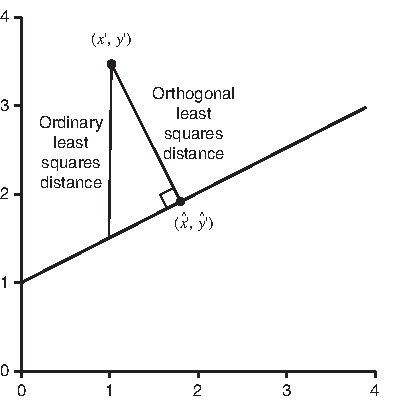
\includegraphics[width=.60\textwidth]{assets/chapter12/fig-12.2.1.pdf}
\caption{正交最小二乘所最小化的距离}\label{fig:12.2.1}
\end{figure}

后面将看到，两个模型有类似问题，并且在某些情形下有类似的似然解. 在结构模型中建立统计理论可能更容易，但在许多情形下函数模型往往显得更合理. 因而，这些内在相似性很有用.

如前所述，两个模型的主要差异之一在于对描述回归关系的参数$\alpha,\beta$的推断. 这种差异极为重要，怎样强调也不过分. 函数关系模型中，给定$\xi_1,\ldots,\xi_n$，利用$X,Y$的条件联合分布进行推断. 结构关系模型中，则利用积分消去$\xi_1,\ldots,\xi_n$后$X,Y$的边际分布，进行不以$\xi_1,\ldots,\xi_n$为条件的推断.

\subsubsection{一种最小二乘解法}\label{sec:12.2.2}\index{SI0609@变量含误差}\index{SI0739@正交最小二乘}
像\autoref{sec:11.3.1}那样，暂时抛开统计，尝试寻找通过观测点$(x_i,y_i)$，$i=1,\ldots,n$的“最佳”直线. 先前假定$x$测量无误差，因此考虑最小化竖直距离是合理的. 这种距离度量隐含假定$x$值正确，得到普通最小二乘（ordinary least squares）. 但这里$x$也有误差，没有理由只考虑竖直距离. 事实上，从统计角度看，普通最小二乘在EIV模型中存在一些问题（见杂录）.

考虑$x$测量也有误差的一种方法，是进行正交最小二乘（orthogonal least squares），即寻找使正交于直线的距离而非竖直距离最小的直线（见\autoref{fig:12.2.1}）. 这种距离度量不像普通最小二乘那样偏向$x$，而是平等对待两个变量. 它也称为总体最小二乘法（total least squares）.\index{SI1035@全最小二乘}\semanticindexanchor{1035:501} 参看\autoref{fig:12.2.1}，对于给定数据点$(x',y')$，在直线$y=a+bx$上按正交距离衡量最近的点由下式给出（\autoref{exercise:12.1}）：
\sourcepageanchor{502}
\begin{equation}\label{eq:12.2.7}
\hat x'=\frac{by'+x'-ab}{1+b^2},\qquad
\hat y'=a+\frac b{1+b^2}(by'+x'-ab).
\end{equation}
现假设有数据$(x_i,y_i)$，$i=1,\ldots,n$. 观测点$(x_i,y_i)$到直线$y=a+bx$上最近点的距离平方为$(x_i-\hat x_i)^2+(y_i-\hat y_i)^2$，其中$\hat x_i,\hat y_i$由\eqref{eq:12.2.7}定义. 总体最小二乘问题是在所有$a,b$上最小化
$$\sum_{i=1}^n\bigl[(x_i-\hat x_i)^2+(y_i-\hat y_i)^2\bigr].$$
容易证明
\begin{equation}\label{eq:12.2.8}
\begin{aligned}
&\sum_{i=1}^n\bigl[(x_i-\hat x_i)^2+(y_i-\hat y_i)^2\bigr]\\
&=\sum_{i=1}^n\left\{\frac{b^2}{(1+b^2)^2}[y_i-(a+bx_i)]^2
+\frac1{(1+b^2)^2}[y_i-(a+bx_i)]^2\right\}\\
&=\frac1{1+b^2}\sum_{i=1}^n(y_i-(a+bx_i))^2.
\end{aligned}
\end{equation}
固定$b$时，和式前的因子为常数. 因而，与\eqref{eq:11.3.9}一样，使和式最小的$a$为$a=\bar y-b\bar x$.\index{SI0610@截距}\semanticindexanchor{610:502} 代回\eqref{eq:12.2.8}，总体最小二乘解就是使
\begin{equation}\label{eq:12.2.9}
\frac1{1+b^2}\sum_{i=1}^n\bigl((y_i-\bar y)-b(x_i-\bar x)\bigr)^2
\end{equation}
在所有$b$上最小的解.

如\eqref{eq:11.3.6}和\eqref{eq:11.3.6}那样，定义平方和与乘积和为\footnote{译注：原文将同一式号11.3.6重复两次；平方和见\eqref{eq:11.3.6}，乘积和见\eqref{eq:11.3.7}. 原重复保留.}
\begin{equation}\label{eq:12.2.10}
\begin{aligned}S_{xx}&=\sum_{i=1}^n(x_i-\bar x)^2,\qquad S_{yy}=\sum_{i=1}^n(y_i-\bar y)^2,\\
S_{xy}&=\sum_{i=1}^n(x_i-\bar x)(y_i-\bar y).
\end{aligned}
\end{equation}
展开平方并求和，\eqref{eq:12.2.9}成为
$$\frac1{1+b^2}\bigl[S_{yy}-2bS_{xy}+b^2S_{xx}\bigr].$$
通常的微积分方法给出最小值（\hyperref[exercise:12.2]{习题12.20}），\footnote{译注：原文引用习题12.20，但该题讨论逻辑回归；这里对应\autoref{exercise:12.2}. 原编号保留.} 得到正交最小二乘直线$y=a+bx$，其中
\begin{equation}\label{eq:12.2.11}\index{SI0612@斜率}
a=\bar y-b\bar x,\qquad b=\frac{-(S_{xx}-S_{yy})+\sqrt{(S_{xx}-S_{yy})^2+4S_{xy}^2}}{2S_{xy}}.
\end{equation}
可以预料，这条直线与最小二乘直线不同. 事实上，后面将看到，它总位于$y$对$x$的普通回归与$x$对$y$的普通回归之间. \autoref{fig:12.2.2}说明了这一点：用\autoref{tab:11.3.1}的数据算得正交最小二乘直线$\hat y=-.49+1.88x$.

简单线性回归中，已看到在正态性假设下，$\alpha,\beta$的普通最小二乘解与MLE相同. 这里，正交最小二乘解只在对参数作出某些假定的特殊情形下才是MLE.

似然估计将遇到的困难，再次表明数学解与统计解的区别. 直线拟合问题的数学最小二乘解并不难获得，似然解却不会如此.

\sourcepageanchor{503}
\begin{figure}[htbp]\centering
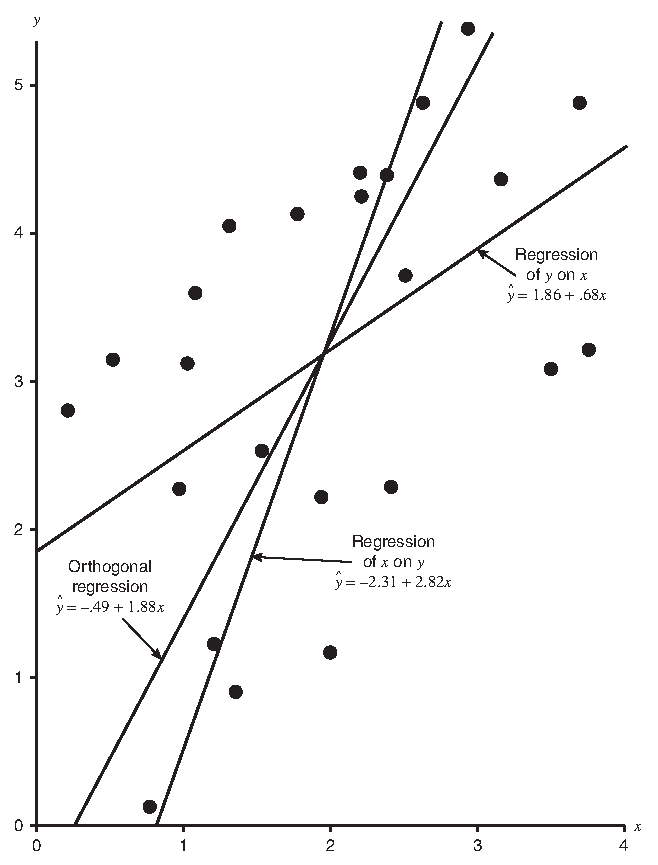
\includegraphics[width=.85\textwidth]{assets/chapter12/fig-12.2.2.pdf}
\caption{\autoref{tab:11.3.1}数据的三条回归直线}\label{fig:12.2.2}
\end{figure}
\subsubsection{最大似然估计}\label{sec:12.2.3}
先考虑函数线性关系模型的最大似然解，结构关系模型的情形类似，并且在某些方面更容易. 利用正态性假设，函数关系模型可表示为
$$Y_i\sim\mathrm n(\alpha+\beta\xi_i,\sigma_\varepsilon^2)
\quad\text{和}\quad X_i\sim\mathrm n(\xi_i,\sigma_\delta^2),\quad i=1,\ldots,n,$$
各$X_i,Y_i$相互独立. 给定观测$(\boldsymbol x,\boldsymbol y)=((x_1,y_1),\allowbreak\ldots,\allowbreak(x_n,y_n))$，似然函数为
\begin{equation}\label{eq:12.2.12}
\begin{aligned}
&L\bigl(\alpha,\beta,\xi_1,\ldots,\xi_n,\sigma_\delta^2,\sigma_\varepsilon^2\mid(\boldsymbol x,\boldsymbol y)\bigr)\\
&=\frac1{(2\pi)^n}\frac1{(\sigma_\delta^2\sigma_\varepsilon^2)^{n/2}}
\exp\left(-\sum_{i=1}^n\frac{(x_i-\xi_i)^2}{2\sigma_\delta^2}\right)
\exp\left(-\sum_{i=1}^n\frac{(y_i-(\alpha+\beta\xi_i))^2}{2\sigma_\varepsilon^2}\right).
\end{aligned}
\end{equation}
\sourcepageanchor{504}
这个似然函数的问题在于没有有限的最大值. 取参数配置$\xi_i=x_i$，再令$\sigma_\delta^2\to0$，函数值便趋于无穷，说明最大似然解不存在. 事实上，\hyperref[bib:source295]{Solari（1969）}证明，若将$L$的一阶导数方程置零并求解，结果是鞍点而非最大值. 注意，只要参数完全由我们控制，就总能迫使似然函数趋于无穷. 特别地，总能使某个方差趋于零，同时让指数项保持有界.

我们作一个常见假设，它既合理，又可缓解许多问题：$\sigma_\delta^2=\lambda\sigma_\varepsilon^2$，其中$\lambda>0$固定且已知. （关于方差的其他假设，见\hyperref[bib:source189]{Kendall和Stuart，1979}，第29章.）这一假设属于限制最少的假设之一，只说已知方差之比，而不知各方差的值. 而且，由此得到的模型具有较好的性质.

在这一假设下，似然函数可写为
\begin{equation}\label{eq:12.2.13}
\begin{aligned}
&L\bigl(\alpha,\beta,\xi_1,\ldots,\xi_n,\sigma_\delta^2\mid(\boldsymbol x,\boldsymbol y)\bigr)\\
&=\frac1{(2\pi)^n}\frac{\lambda^{n/2}}{(\sigma_\delta^2)^n}
\exp\left[-\sum_{i=1}^n\frac{(x_i-\xi_i)^2+\lambda(y_i-(\alpha+\beta\xi_i))^2}{2\sigma_\delta^2}\right],
\end{aligned}
\end{equation}
现在可以将它最大化. 将分阶段最大化，确保每一步都得到最大值后再进行下一步. 考察\eqref{eq:12.2.13}，可以确定合理的最大化顺序.

首先，对每个$\alpha,\beta,\sigma_\delta^2$值，为使$L$关于$\xi_1,\ldots,\xi_n$最大，最小化$\sum_{i=1}^n\bigl((x_i-\xi_i)^2+\lambda(y_i-(\alpha+\beta\xi_i))^2\bigr)$. （细节见\autoref{exercise:12.3}.）对每个$i$，这是$\xi_i$的二次式，最小值在
$$\xi_i^*=\frac{x_i+\lambda\beta(y_i-\alpha)}{1+\lambda\beta^2}$$
处取得. 代回得到
$$\sum_{i=1}^n\bigl((x_i-\xi_i^*)^2+\lambda(y_i-(\alpha+\beta\xi_i^*))^2\bigr)
=\frac\lambda{1+\lambda\beta^2}\sum_{i=1}^n(y_i-(\alpha+\beta x_i))^2.$$
似然函数现在成为
\begin{equation}\label{eq:12.2.14}
\begin{aligned}
&\max_{\xi_1,\ldots,\xi_n}L(\alpha,\beta,\xi_1,\ldots,\xi_n,\sigma_\delta^2\mid(\boldsymbol x,\boldsymbol y))\\
&=\frac1{(2\pi)^n}\frac{\lambda^{n/2}}{(\sigma_\delta^2)^n}
\exp\left\{-\frac1{2\sigma_\delta^2}\left[\frac\lambda{1+\lambda\beta^2}\sum_{i=1}^n(y_i-(\alpha+\beta x_i))^2\right]\right\}.
\end{aligned}
\end{equation}
现在可以关于$\alpha,\beta$最大化，但稍加计算就会发现，已经在正交最小二乘解中做过这件事了！确实，EIV模型的正交最小二乘与最大似然之间存在某种对应，下面就利用它. 定义
\begin{equation}\label{eq:12.2.15}
\alpha^*=\sqrt\lambda\alpha,\quad\beta^*=\sqrt\lambda\beta,\quad
y_i^*=\sqrt\lambda y_i,\quad i=1,\ldots,n.
\end{equation}
\eqref{eq:12.2.14}中的指数部分成为
$$\frac\lambda{1+\lambda\beta^2}\sum_{i=1}^n(y_i-(\alpha+\beta x_i))^2
=\frac1{1+\beta^{*2}}\sum_{i=1}^n(y_i^*-(\alpha^*+\beta^*x_i))^2,$$
\sourcepageanchor{505}
这与正交最小二乘问题中的表达式相同. 由\eqref{eq:12.2.11}知道使其最小的$\alpha^*,\beta^*$，再利用\eqref{eq:12.2.15}，得到截距和斜率的MLE：
\begin{equation}\label{eq:12.2.16}\index{SI0413@函数型}
\hat\alpha=\bar y-\hat\beta\bar x\quad\text{和}\quad
\hat\beta=\frac{-(S_{xx}-\lambda S_{yy})+\sqrt{(S_{xx}-\lambda S_{yy})^2+4\lambda S_{xy}^2}}{2\lambda S_{xy}}.
\end{equation}
从公式可见，当$\lambda=1$时，MLE与正交最小二乘解一致. 这很合理：正交最小二乘把$x,y$当作具有相同大小的误差，即方差比为1. 将这一论证推进一步，可把此解与假定$x$固定时的普通最小二乘或最大似然联系起来. 若$x$固定，其方差为零，因而$\lambda=0$. 一般$\lambda$下的最大似然解在这种情形下确实退化为普通最小二乘解. \autoref{exercise:12.4}探讨这一关系及其他关系.

将\eqref{eq:12.2.16}与\eqref{eq:12.2.14}结合，似然几乎已完全最大化. 有
\begin{equation}\label{eq:12.2.17}
\begin{aligned}
&\max_{\alpha,\beta,\xi_1,\ldots,\xi_n}L(\alpha,\beta,\xi_1,\ldots,\xi_n,\sigma_\delta^2\mid(\boldsymbol x,\boldsymbol y))\\
&=\frac1{(2\pi)^n}\frac{\lambda^{n/2}}{(\sigma_\delta^2)^n}
\exp\left[-\frac1{2\sigma_\delta^2}\frac\lambda{1+\lambda\hat\beta^2}\sum_{i=1}^n\bigl(y_i-(\hat\alpha+\hat\beta x_i)\bigr)^2\right].
\end{aligned}
\end{equation}
现在关于$\sigma_\delta^2$最大化$L$，与通常正态抽样中求$\sigma^2$的MLE非常相似（\autoref{ex:7.2.11}），主要差异在于$\sigma_\delta^2$的指数为$n$而非$n/2$. 细节留给\autoref{exercise:12.5}. 得到$\sigma_\delta^2$的MLE为
\begin{equation}\label{eq:12.2.18}
\hat\sigma_\delta^2=\frac1{2n}\frac\lambda{1+\lambda\hat\beta^2}\sum_{i=1}^n\bigl(y_i-(\hat\alpha+\hat\beta x_i)\bigr)^2.
\end{equation}
由MLE的性质，$\sigma_\varepsilon^2$的MLE为$\hat\sigma_\varepsilon^2=\hat\sigma_\delta^2/\lambda$，并且$\hat\xi_i=\hat\alpha+\hat\beta x_i$.\footnote{译注：原文此处将$\hat\xi_i$写成拟合响应. 根据前一页对$\xi_i$的最大化，实际应为$[x_i+\lambda\hat\beta(y_i-\hat\alpha)]/(1+\lambda\hat\beta^2)$. 原式保留.} 尽管通常不关心$\hat\xi_i$，但需要预测时它们有时会有用. 此外，$\hat\xi_i$也可用于检验拟合是否充分（见\hyperref[bib:source130]{Fuller，1987）}.

有趣的是，虽然$\hat\alpha,\hat\beta$是相合估计量，$\sigma_\delta^2$却不是.\index{SI0409@相合性}\semanticindexanchor{409:505}\index{SI0675@变量含误差}\semanticindexanchor{675:505}\footnote{译注：此处讨论估计量的相合性，原文$\sigma_\delta^2$应指$\hat\sigma_\delta^2$，下式也如此表明. 原符号保留.} 更确切地说，当$n\to\infty$时，
$$\hat\alpha\to\alpha\quad\text{依概率},\qquad\hat\beta\to\beta\quad\text{依概率},$$
但
$$\hat\sigma_\delta^2\to\tfrac12\sigma_\delta^2\quad\text{依概率}.$$
\hyperref[bib:source143]{Gleser（1981）}给出了EIV函数关系模型中相合性的一般结果.

现在转向线性结构关系模型.\index{SI0415@结构型}\semanticindexanchor{415:505} 回顾这里假设按照
$$\begin{aligned}Y_i&\sim\mathrm n(\alpha+\beta\xi_i,\sigma_\varepsilon^2),\\
X_i&\sim\mathrm n(\xi_i,\sigma_\delta^2),\\
\xi_i&\sim\mathrm n(\xi,\sigma_\xi^2),
\end{aligned}$$
观测$(X_i,Y_i)$，$i=1,\ldots,n$，其中$\xi_i$相互独立，给定$\xi_i$时，各$X_i,Y_i$相互独立. 如前，对$\alpha,\beta$的推断将使用$X_i,Y_i$的边际分布，即积分消去$\xi_i$所得的分布.
\sourcepageanchor{506}
积分消去$\xi_i$，得到$(X_i,Y_i)$的边际分布（\autoref{exercise:12.6}）：
\begin{equation}\label{eq:12.2.19}
(X_i,Y_i)\sim\text{二元正态}\bigl(\xi,\alpha+\beta\xi,\sigma_\delta^2+\sigma_\xi^2,
\sigma_\varepsilon^2+\beta^2\sigma_\xi^2,\beta\sigma_\xi^2\bigr).
\end{equation}
注意这一相关结构与RCB ANOVA\index{SI0416@与随机完全区组的关系}\semanticindexanchor{416:506}\index{SI0875@与变量含误差的关系}\semanticindexanchor{875:506}（\hyperref[sec:11.5.3]{杂录11.5.3}）的相似之处. 在那里，给定区组时观测不相关，但无条件时存在组内相关. 这里，以$\xi_i$为条件的函数关系模型的观测不相关，但在不以$\xi_i$为条件作推断的结构关系模型中，观测相关. $\xi_i$起着类似区组的作用，这里的相关类似于组内相关. （事实上，若$\beta=1$且$\sigma_\delta^2=\sigma_\varepsilon^2$，它就等于组内相关.）

在这种情形下作似然估计，给定观测$(\boldsymbol x,\boldsymbol y)=((x_1,y_1),\allowbreak\ldots,\allowbreak(x_n,y_n))$，似然函数是二元正态的似然，如\autoref{exercise:7.18}中所见. 在那里，二元正态的似然估计可通过令样本量等于总体量求得. 因此，为求$\alpha,\beta,\xi,\sigma_\varepsilon^2,\sigma_\delta^2,\sigma_\xi^2$的MLE，解方程
\begin{equation}\label{eq:12.2.20}
\begin{aligned}
\bar y&=\hat\alpha+\hat\beta\hat\xi,&\bar x&=\hat\xi,\\
\frac1nS_{yy}&=\hat\sigma_\varepsilon^2+\hat\beta^2\hat\sigma_\xi^2,\\
\frac1nS_{xx}&=\hat\sigma_\delta^2+\hat\sigma_\xi^2,\\
\frac1nS_{xy}&=\hat\beta\hat\sigma_\xi^2.
\end{aligned}
\end{equation}
五个方程却有六个未知数，所以方程组不定. 即方程组没有唯一解，使似然最大的参数向量$(\alpha,\beta,\xi,\sigma_\varepsilon^2,\sigma_\delta^2,\sigma_\xi^2)$也没有唯一取值.

继续之前，须认识到这里$X_i,Y_i$的方差与函数关系模型中的方差不同. 在那里，以$\xi_1,\ldots,\xi_n$为条件；这里则对$\xi_i$取边际分布. 例如，函数关系模型中写$\operatorname{Var}X_i=\sigma_\delta^2$，隐含这是给定$\xi_1,\ldots,\xi_n$的条件方差；结构模型中写$\operatorname{Var}X_i=\sigma_\delta^2+\sigma_\xi^2$，隐含这是不以$\xi_1,\ldots,\xi_n$为条件的方差. 不应因此产生混淆.

\eqref{eq:12.2.20}的解对$\hat\beta$施加一个限制，函数关系情形中已经遇到这个限制（\autoref{exercise:12.4}）. 由上述方差与协方差方程，容易推得
$$\begin{aligned}
\hat\sigma_\delta^2\ge0&\quad\text{仅当}\quad S_{xx}\ge\frac1{\hat\beta}S_{xy},\\
\hat\sigma_\varepsilon^2\ge0&\quad\text{仅当}\quad S_{yy}\ge\hat\beta S_{xy},
\end{aligned}$$
二者共同推出
$$\frac{|S_{xy}|}{S_{xx}}\le|\hat\beta|\le\frac{S_{yy}}{|S_{xy}|}.$$
（\autoref{exercise:12.9}建立$\hat\beta$的界.）

现在处理结构关系情形中的可识别性问题.\index{SI0411@可识别性}\semanticindexanchor{411:506}\index{SI0528@变量含误差}\semanticindexanchor{528:506} 这个问题并不意外，因为\eqref{eq:12.2.19}中的参数数目多于确定分布所需的数目. 要使结构线性关系模型可识别，必须作一个假设，把参数数目减少到五个. 幸运的是，对函数关系所作的方差假设也能解决这里的可识别性问题.
\sourcepageanchor{507}
因此，假设$\sigma_\delta^2=\lambda\sigma_\varepsilon^2$，其中$\lambda$已知. 这使未知参数数目降到五个，使模型可识别（见\autoref{exercise:12.8}）. 更强的限制，如假设$\sigma_\delta^2$已知，可能导致方差的MLE取零值. \hyperref[bib:source189]{Kendall和Stuart（1979}，第29章）对此有完整讨论.

一旦假设$\sigma_\delta^2=\lambda\sigma_\varepsilon^2$，本模型中$\hat\alpha,\hat\beta$的最大似然估计便与函数关系模型相同，由\eqref{eq:12.2.16}给出. 但方差估计不同，为
\begin{equation}\label{eq:12.2.21}
\begin{aligned}
\hat\sigma_\delta^2&=\frac1n\left(S_{xx}-\frac{S_{xy}}{\hat\beta}\right),\\
\hat\sigma_\varepsilon^2&=\frac{\hat\sigma_\delta^2}\lambda=\frac1n(S_{yy}-\hat\beta S_{xy}),\\
\hat\sigma_\xi^2&=\frac1n\frac{S_{xy}}{\hat\beta}.
\end{aligned}
\end{equation}
（\autoref{exercise:12.10}证明这些结果，并探讨这里的方差估计与函数模型中的方差估计之间的关系.）注意，与函数关系模型不同，在线性结构关系模型中，这些估计量全都相合\index{SI0409@相合性}\semanticindexanchor{409:507}\index{SI0675@变量含误差}\semanticindexanchor{675:507}（当$\sigma_\delta^2=\lambda\sigma_\varepsilon^2$时）.

\subsubsection{置信集}\label{sec:12.2.4}\index{SI0182@变量含误差}\index{SI0408@置信集}
可以预料，EIV模型中构造置信集是困难的. 完整讨论需要本书尚未建立的工具. 这里仅集中于斜率$\beta$的置信集.

首先，可用\autoref{sec:10.4.1}的近似似然方法构造近似置信区间. 实践中这可能是最常见的做法，也并非全无道理. 但是，这些近似区间不能保持名义$1-\alpha$置信水平. 事实上，\hyperref[bib:source150]{Gleser和Hwang（1987）}的结果给出一个令人不安的结论：任何长度始终有限的斜率区间估计量，其置信系数都等于零！

为明确起见，本节余下部分假定采用EIV模型的结构关系情形. 所给置信集结果对结构与函数两种情形都有效，尤其公式保持相同. 继续假定$\sigma_\delta^2=\lambda\sigma_\varepsilon^2$，其中$\lambda$已知.

\hyperref[bib:source150]{Gleser和Hwang（1987）}指出，参数
$$\tau^2=\frac{\sigma_\xi^2}{\sigma_\delta^2}$$
决定数据中为确定斜率$\beta$而可能提供的信息量. 他们证明，当$\tau^2\to0$时，任何有限长度的$\beta$置信区间，其覆盖概率也必趋于0. 要理解这为何合理，注意$\tau^2=0$意味着$\xi_i$没有变动，从而不可能拟合唯一的直线.

可利用以下事实构造$\beta$的近似置信区间：估计量
$$\hat\sigma_\beta^2=\frac{(1+\lambda\hat\beta^2)^2(S_{xx}S_{yy}-S_{xy}^2)}{(S_{xx}-\lambda S_{yy})^2+4\lambda S_{xy}^2}$$
是$\hat\beta$的真实方差$\sigma_\beta^2$的相合估计量.\footnote{译注：结合下式除以$\sqrt n$的标准误，这里的$\sigma_\beta^2$应理解为$\sqrt n(\hat\beta-\beta)$的渐近方差，而非$\hat\beta$本身的有限样本方差. 原表述保留.} 因而，结合中心极限定理与Slutsky定理（\autoref{sec:5.5}），可证明区间
$$\hat\beta-\frac{z_{\alpha/2}\hat\sigma_\beta}{\sqrt n}\le\beta\le
\hat\beta+\frac{z_{\alpha/2}\hat\sigma_\beta}{\sqrt n}$$
\sourcepageanchor{508}
是$\beta$的近似$1-\alpha$置信区间. 但因为长度有限，它无法对所有参数值保持$1-\alpha$覆盖率.

\hyperref[bib:source145]{Gleser（1987）}考虑了这一区间的一种修正，并将其覆盖概率的下确界报告为$\tau^2$的函数. Gleser的修正$C_G(\hat\beta)$为
\begin{equation}\label{eq:12.2.22}
\hat\beta-\frac{t_{n-2,\alpha/2}\hat\sigma_\beta}{\sqrt{n-2}}\le\beta\le
\hat\beta+\frac{t_{n-2,\alpha/2}\hat\sigma_\beta}{\sqrt{n-2}}.
\end{equation}
再利用中心极限定理与Slutsky定理，可证明这是$\beta$的近似$1-\alpha$置信区间. 因为这个区间的长度也有限，同样无法对所有参数值保持$1-\alpha$覆盖率. Gleser作了若干有限样本数值计算，给出覆盖概率下确界作为$\tau^2$函数的界. 对合理大小的$n$（$\ge10$），若$\tau^2\ge.25$，名义90\%区间的覆盖概率至少为80\%. 随$\tau^2$或$n$增加，表现会改善.

\eqref{eq:12.2.22}的$C_G(\hat\beta)$长度有限，却不保证覆盖概率；现在考察一个精确置信集，按其必须具有的性质，它的长度无穷.\footnote{译注：结合下文可由两个有限区间组成的情形，这里应理解为置信集不能始终具有有限长度，而非每个样本得到的集合都长为无穷. 原表述保留.} 这个集合称为Creasy--Williams置信集，由\hyperref[bib:source87]{Creasy（1956）}及\hyperref[bib:source331]{Williams（1959）}提出，依据以下事实（见\autoref{exercise:12.11}）：若$\sigma_\delta^2=\lambda\sigma_\varepsilon^2$，则
$$\operatorname{Cov}(\beta\lambda Y_i+X_i,Y_i-\beta X_i)=0.$$
定义$r_\lambda(\beta)$为$\beta\lambda Y_i+X_i$与$Y_i-\beta X_i$的样本相关系数，即\footnote{译注：原式第二行分母最后一项为$-\beta^2S_{xx}$；展开第一行第二个平方和可知应为$+\beta^2S_{xx}$. 原式保留.}
\begin{equation}\label{eq:12.2.23}
\begin{aligned}
r_\lambda(\beta)
&=\frac{\sum_{i=1}^n((\beta\lambda y_i+x_i)-(\beta\lambda\bar y+\bar x))((y_i-\beta x_i)-(\bar y-\beta\bar x))}
{\sqrt{\sum_{i=1}^n((\beta\lambda y_i+x_i)-(\beta\lambda\bar y+\bar x))^2\sum_{i=1}^n((y_i-\beta x_i)-(\bar y-\beta\bar x))^2}}\\
&=\frac{\beta\lambda S_{yy}+(1-\beta^2\lambda)S_{xy}-\beta S_{xx}}
{\sqrt{(\beta^2\lambda^2S_{yy}+2\beta\lambda S_{xy}+S_{xx})(S_{yy}-2\beta S_{xy}-\beta^2S_{xx})}}.
\end{aligned}
\end{equation}
因为$\beta\lambda Y_i+X_i$与$Y_i-\beta X_i$服从相关系数为零的二元正态分布，由\autoref{exercise:11.33}有
$$\frac{\sqrt{n-2}\,r_\lambda(\beta)}{\sqrt{1-r_\lambda^2(\beta)}}\sim t_{n-2},$$
对任何$\beta$值都成立. 因而找到一个枢轴量，并得出集合
\begin{equation}\label{eq:12.2.24}\index{SI0186@变量含误差}
\left\{\beta:\frac{(n-2)r_\lambda^2(\beta)}{1-r_\lambda^2(\beta)}\le F_{1,n-2,\alpha}\right\}
\end{equation}
是$\beta$的$1-\alpha$置信集（见\autoref{exercise:12.11}）.

尽管这是$1-\alpha$置信集，它有类似于Fieller区间的缺点. 描述集合\eqref{eq:12.2.24}的函数有两个极小值，函数值均为零. 置信集可以由两个有限的不相交区间、一个有限和两个无限的不相交区间组成，也可能是整个实轴. 例如，\autoref{tab:11.3.1}的数据在$\lambda=1$时，$F$统计量函数的图形见\autoref{fig:12.2.3}. 置信集包含使函数值小于等于$F_{1,22,\alpha}$的所有$\beta$. 当$\alpha=.05$、$F_{1,22,.05}=4.30$时，置信集为$[-1.13,-.14]\cup[.89,7.38]$. 当$\alpha=.01$、$F_{1,22,.01}=7.95$时，置信集为$(-\infty,-18.18]\cup[-1.68,.06]\cup[.60,\infty)$.

此外，对每个$\beta$，$-r_\lambda(\beta)=r_\lambda(-1/(\lambda\beta))$（见\autoref{exercise:12.12}），所以若$\beta$在置信集中，$-1/(\lambda\beta)$也在其中. 这一置信集不能区分$\beta$与$-1/(\lambda\beta)$，始终同时包含正值和负值. 我们永远不能由这个置信集确定斜率的符号！

\eqref{eq:12.2.24}的置信集并非\hyperref[bib:source87]{Creasy（1956）}原来讨论的那个，而是其修正. 她实际关心估计的是$\beta$与$x$轴所成的角$\phi$，即$\beta=\tan(\phi)$，相应置信集的问题较少.
\sourcepageanchor{509}
在EIV模型中，估计$\phi$也许更自然（例如见\hyperref[bib:source4]{Anderson，1976）}，但我们似乎更倾向于估计$\alpha,\beta$.

\begin{figure}[htbp]\centering
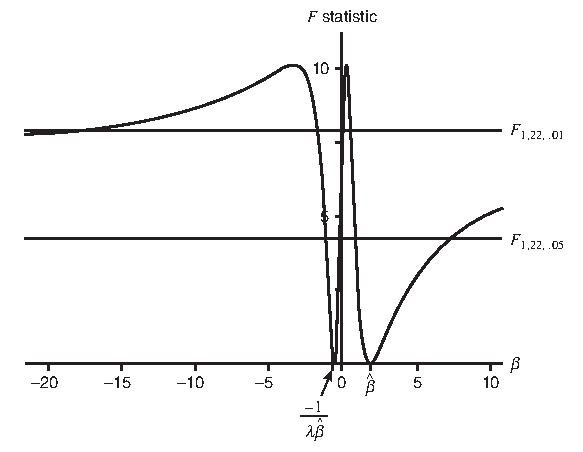
\includegraphics[width=.78\textwidth]{assets/chapter12/fig-12.2.3.pdf}
\caption{定义Creasy--Williams置信集的$F$统计量，$\lambda=1$}\label{fig:12.2.3}
\end{figure}
普通线性回归中能进行的其他标准统计分析，大多数在EIV模型中也有对应方法. 例如，可以检验关于$\beta$的假设，或估计$EY_i$的值. 更多内容见\hyperref[bib:source130]{Fuller（1987）}或\hyperref[bib:source189]{Kendall和Stuart（1979}，第29章）.
